\ProvidesFile{lecture27.tex}[Лекция 27]


\subsection{Геометрический смысл Сигнатуры}

\begin{claim}
Пусть $V$ -- векторное пространство над $\mathbb R$ и $\beta\colon V\times V\to \mathbb R$ -- симметричная билинейная форма на $V$.
\begin{enumerate}
\item Пусть $W\subseteq V$ -- максимальное по вложению подпространство такое, что $\beta(w, w) > 0$ для любого ненулевого $w\in W$.
Тогда $\#1 = \dim W$.

\item Пусть $W\subseteq V$ -- максимальное по вложению подпространство такое, что $\beta(w, w) < 0$ для любого ненулевого $w\in W$.
Тогда $\#-1 = \dim W$.
\end{enumerate}
\end{claim}
\begin{proof}
Если заменить форму $\beta$ на $-\beta$, то количество единиц в сигнатуре $-\beta$ равно количеству минус единиц в сигнатуре $\beta$.
Потому достаточно доказать только первое утверждение.


Так как $\beta(w, w) > 0$ для любого ненулевого $w\in W$, то $\beta|_W$ не вырождена, а значит $V = W\oplus W^\bot$  по утверждению~\ref{claim::NonDegRestrictionBil} пункт~2.
Пусть $e_1,\ldots,e_k$ -- базис $W$, в котором $\beta|_W$ диагональная с единицами на диагонали.
Так же выберем $e_{k+1},\ldots,e_n$ базис $W^\bot$, в котором $\beta|_{W^\bot}$ диагонализуема с единицами, минус единицами и нулями на диагонали.
Если в сигнатуре $\beta|_{W^\bot}$ есть хотя бы одна единица, например на $k+1$ месте, то на подпространстве $W+\langle e_{k+1}\rangle$ в базисе $e_1,\ldots,e_{k+1}$ форма $\beta$ задана в виде $\beta(x, y) = x^t y$ и потому $\beta(x,x)$ положительна для любого ненулевого вектора, что противоречит выбору $W$.
Значит в сигнатуре $\beta|_{W^\bot}$ могут быть только $-1$ и $0$.
А значит в сигнатуре $\beta$ единицы взялись только из блока для $\beta|_W$, что завершает доказательство.
\end{proof}

\paragraph{Замечания}

\begin{itemize}
\item Стоит отметить, что аналог формулы из предыдущего утверждения не подходит для вычисления $\#0$.
Например, если взять $\beta\colon \mathbb R^2 \times \mathbb R^2 \to \mathbb R$ заданную матрицей $\left(\begin{smallmatrix}{0}&{1}\\{1}&{0}\end{smallmatrix}\right)$, то для $W = \langle e_1\rangle$ выполнено $\beta|_W = 0$.
Однако, форма $\beta$ невырождена, а значит $\#0 = 0$.
В этом случае $\#0$ надо искать как размерность ядра формы.

\item Аналогично можно показать следующее утверждение.
Если $\beta\colon V\times V\to \mathbb R$ -- симметричная билинейная форма, $U\subseteq V$ -- подпространство такое, что $\beta|_U$ невырождена, тогда $\# 1$ для $\beta$ не меньше, чем $\# 1$ для $\beta|_W$ и $\#-1$ для $\beta$ не меньше, чем $\#-1$ для $\beta|_W$.
\end{itemize}

\begin{claim}
Пусть $V$ -- векторное пространство над $\mathbb R$ и $\beta\colon V\times V\to \mathbb R$ -- симметричная билинейная форма на $V$.
Пусть $W\subseteq V$ -- максимальное по вложению подпространство такое, что $\beta|_W = 0$.
Тогда $\dim W = \min(\#1, \#-1) + \#0$.
\end{claim}
\begin{proof}
Обратите внимание, что $\ker \beta \subseteq W$.
Действительно, если это не  так, то на подпространстве $W+\ker \beta$ форма $\beta$ полностью нулевая, но это подпространство больше по включению.
Теперь выберем базис пространства $V$ следующим образом: в начале возьмем $e_1,\ldots,e_k \in \ker \beta$ -- базис ядра.
Потом дополним его до базиса $W$ векторами $e_{k+1},\ldots,e_{k+m}$.
Пусть $U = \langle e_{k+1},\ldots,e_{k+m}\rangle$.
Тогда $W = \ker \beta \oplus U$.
Так же дополним $W$ прямым слагаемым до всего подпространства $V$, то есть найдем такое $E\subseteq V$, что $V = W \oplus E$.

Заметим, что ограничение $\beta'\colon U\times E \to \mathbb R$ не имеет левого ядра.
Действительно, если у этой формы есть левое ядро, то эти векторы лежат в ядре $\beta$, которое не пересекается с $U$, противоречие.
Значит, мы можем найти в $E$ подпространство $U'$ такой же размерности, что и $U$ такие, что ограничение $\beta$ на $U\times U'$ будет невырожденной.
А значит, мы можем выбрать базис в $U$ и $U'$ так, что матрица в нем будет иметь вид
\[
\begin{pmatrix}
{\beta|_{U}}&{\beta|_{U\times U'}}\\
{\beta|_{U'\times U}}&{\beta|_{U'}}\\
\end{pmatrix}
=
\begin{pmatrix}
{0}&{E}\\
{E}&{*}
\end{pmatrix}
\]
Симметричным гауссом вычитая более верхние строки из более нижних и более левые столбцы из более правых, мы можем занулить блок справа внизу.
Значит можно так поменять базис, что
\[
\begin{pmatrix}
{\beta|_{U}}&{\beta|_{U\times \bar U}}\\
{\beta|_{\bar U\times U}}&{\beta|_{\bar U}}\\
\end{pmatrix}
=
\begin{pmatrix}
{0}&{E}\\
{E}&{0}
\end{pmatrix}
\]
для некоторого нового подпространства $\bar U$.

На подпространстве $U\oplus E$ форма $\beta$ не вырождена, а значит $U\oplus E = U \oplus \bar U \oplus(U \oplus \bar U)^\bot$ по утверждению~\ref{claim::NonDegRestrictionBil} пункт~(2).
В итоге мы выбрали базис в $U\oplus \bar U$ так, что матрица билинейной формы на этом подпространстве имеет вид
\[
\begin{pmatrix}
{0}&{E}\\
{E}&{0}
\end{pmatrix}
\]
А значит, выбрав базис в ортогональном дополнении и в ядре, мы получим, что матрица для $\beta$ имеет вид
\[
B_\beta = 
\begin{pmatrix}
{0}&{0}&{0}&{0}\\
{0}&{0}&{E}&{0}\\
{0}&{E}&{0}&{0}\\
{0}&{0}&{0}&{C}\\
\end{pmatrix}
\]
При этом $W$ порождено базисными векторами соответствующим первым двум блокам.

Теперь мы можем допривести полученную матрицу к диагональному виду.
В перестановкой базисных векторов можно сделать
\[
\begin{pmatrix}
{0}&{E}\\
{E}&{0}\\
\end{pmatrix}
\mapsto
\begin{pmatrix}
{0}&{1}&{}&{}&{}\\
{1}&{0}&{}&{}&{}\\
{}&{}&{0}&{1}&{}\\
{}&{}&{1}&{0}&{}\\
{}&{}&{}&{}&{\ddots}\\
\end{pmatrix}
\]
А теперь мы видим, что у каждого блока $2$ на $2$ сигнатура состоит из одной единицы и одной минус единицы.
Далее мы доприводим блок $C$ к диагональному виду.
Получаем
\[
B_\beta =
\begin{pmatrix}
{0}&{}&{}&{}&{}\\
{}&{E}&{}&{}&{}\\
{}&{}&{-E}&{}&{}\\
{}&{}&{}&{E}&{}\\
{}&{}&{}&{}&{-E}\\
\end{pmatrix}
\]
Здесь последние два блока взялись из матрицы $C$.
Откуда мы видим, что размерность $W$ не больше $\#0 + \min(\#1, \#-1)$.
Давайте покажем, что если размерность $W$ строго меньше, то мы можем его увеличить.
Если размерность строго меньше, то это значит, что в сигнатуре $C$ есть и единицы и минус единицы.
Вернемся к базису, в котором матрица билинейной формы имеет вид
\[
B_\beta = 
\begin{pmatrix}
{0}&{0}&{0}&{0}\\
{0}&{0}&{E}&{0}\\
{0}&{E}&{0}&{0}\\
{0}&{0}&{0}&{C}\\
\end{pmatrix}
\]
Пусть $U$ -- подпространство, на котором билинейная форма задана матрицей $C$.
Так как в сигнатуре $C$ есть и единицы и минус единицы, мы можем выбрать в $C$ два ортогональных вектора $f$ и $g$ такие, что $\beta(f,f) = 1$ и $\beta(g,g) = -1$.
Тогда можно проверить, что на подпространстве $W + \langle f + g\rangle$ форма $\beta$ будет тождественно нулем.
А это противоречит максимальности $W$.
Это противоречие возникло из предположения, что $\dim W < \#0 + \min(\#1, \#-1)$.
\end{proof}

\subsection{Положительная и отрицательная определенность формы над $\mathbb R$}

\begin{definition}
Пусть $\beta\colon V\times V\to \mathbb R$ -- симметричная билинейная форма.
Тогда
\begin{itemize}
\item $\beta$ (или $Q_\beta$) называется положительно определенной (или кратко положительной), если $Q_\beta(v) > 0$ для любого $v\neq 0$, $v\in V$.

\item $\beta$ (или $Q_\beta$) называется отрицательно определенной (или кратко отрицательной), если $Q_\beta(v) < 0$ для любого $v\neq 0$, $v\in V$.

\item $\beta$ (или $Q_\beta$) называется неотрицательно определенной (или кратко неотрицательной), если $Q_\beta(v) \geqslant 0$ для любого $v\in V$.

\item $\beta$ (или $Q_\beta$) называется неположительно определенной (или кратко неположительной), если $Q_\beta(v) \leqslant 0$ для любого $v\in V$.

\item В противном случае $\beta$ и $Q_\beta$ называются неопределенными.
\end{itemize}
\end{definition}

\paragraph{Замечание}

Обратите внимание, что определение зависит от значений квадратичной формы, а не самой билинейной формы.
То есть $\beta(u,v)$ может быть вообще говоря каким угодно (если $\beta(u, v) >0$, то $\beta(-u, v)< 0$), а мы смотрим на $\beta(v, v)$.

Ниже я все определения отразил в единой табличке.
В ней подразумевается, что билинейная форма задана на пространстве размерности $n$.
\begin{center}
\begin{tabular}{|c|c|c|c|}
\hline
{\bf Термин}&{\bf Обозначения}&{\bf Условие}&{\bf Индексы}\\
\hline
{Положительная}&{$\beta>0$ или $Q>0$}&{$\forall x\neq 0\Rightarrow Q(x) > 0$}&{$\# 1 = n$}\\
\hline
{Отрицательная}&{$\beta<0$ или $Q<0$}&{$\forall x\neq 0\Rightarrow Q(x) < 0$}&{$\#-1 = n$}\\
\hline
{Неотрицательная}&{$\beta\geqslant0$ или $Q\geqslant0$}&{$\forall x\Rightarrow Q(x) \geqslant 0$}&{$\#-1 = 0$}\\
\hline
{Неположительная}&{$\beta\leqslant0$ или $Q\leqslant0$}&{$\forall x\Rightarrow Q(x) \leqslant 0$}&{$\#1 = 0$}\\
\hline
{Неопределенная}&{}&{$\exists x, y\Rightarrow Q(x) > 0$ и $Q(y)<0$}&{$\#1>0$ и $\#-1>0$}\\
\hline
\end{tabular}
\end{center}

\begin{claim}
[Критерий Сильвестра]
\label{claim::SilvCrit}
Пусть $\beta\colon V\times V\to \mathbb R$ -- симметрическая билинейная форма и пусть в некотором базисе $e_1,\ldots,e_n$ она записывается в виде $\beta(x, y) = x^t B y$, где $B\in \operatorname{M}_n(\mathbb R)$ -- симметрическая матрица.
Обозначим ее угловые миноры через $\Delta_1,\ldots,\Delta_n$.
Тогда
\begin{enumerate}
\item Форма $\beta$ положительно определена тогда и только тогда, когда $\Delta_i > 0$ для любого $i$.

\item Форма $\beta$ отрицательно определена тогда и только тогда, когда $\sgn \Delta_i = (-1)^i$.
\end{enumerate}
\end{claim}
\begin{proof}
(1) Пусть $W = \langle e_1,\ldots,e_i\rangle$.
Если $\beta$ положительно определена, то $\beta|_W$ тоже положительно определена.
Кроме того $\Delta_i = \det \beta|_W$.
Так как над полем $\mathbb R$ знак определителя формы не зависит от базиса (раздел~\ref{subsection::BilChar}), то достаточно посчитать этот определитель в удобном базисе.
Так как $\beta|_W$ положительно определена, то $\#1 = n$, то есть в каком то базисе она задана единичной матрицей.

Обратно, пусть $\Delta_i > 0$.
Тогда можно применить алгоритм Якоби.
Значит форма приводится к диагональному виду с числами $\Delta_1, \Delta_2/\Delta_1,\ldots,\Delta_n/\Delta_{n-1}$ на диагонали.
Значит $\#1 = n$, то есть форма положительно определена.

(2) Заметим, что $\beta$ отрицательно определена тогда и только тогда, когда $-\beta$ положительно определена.
Тогда $\sgn\Delta_i(-\beta) = (-1)^i\sgn\Delta_i(\beta)$.
Теперь утверждение следует из первого пункта.
\end{proof}

\subsection{Графики Квадратичных форм}

Пусть $V = \mathbb R^2$.
Тогда квадратичная форма $Q(x, y)$ задает функцию от двух переменных.
Давайте нарисуем ее графики в различных ситуациях.

\begin{enumerate}
\item Положительно определенная форма $z = x^2 + y^2$.
Начало координат -- точка минимума.

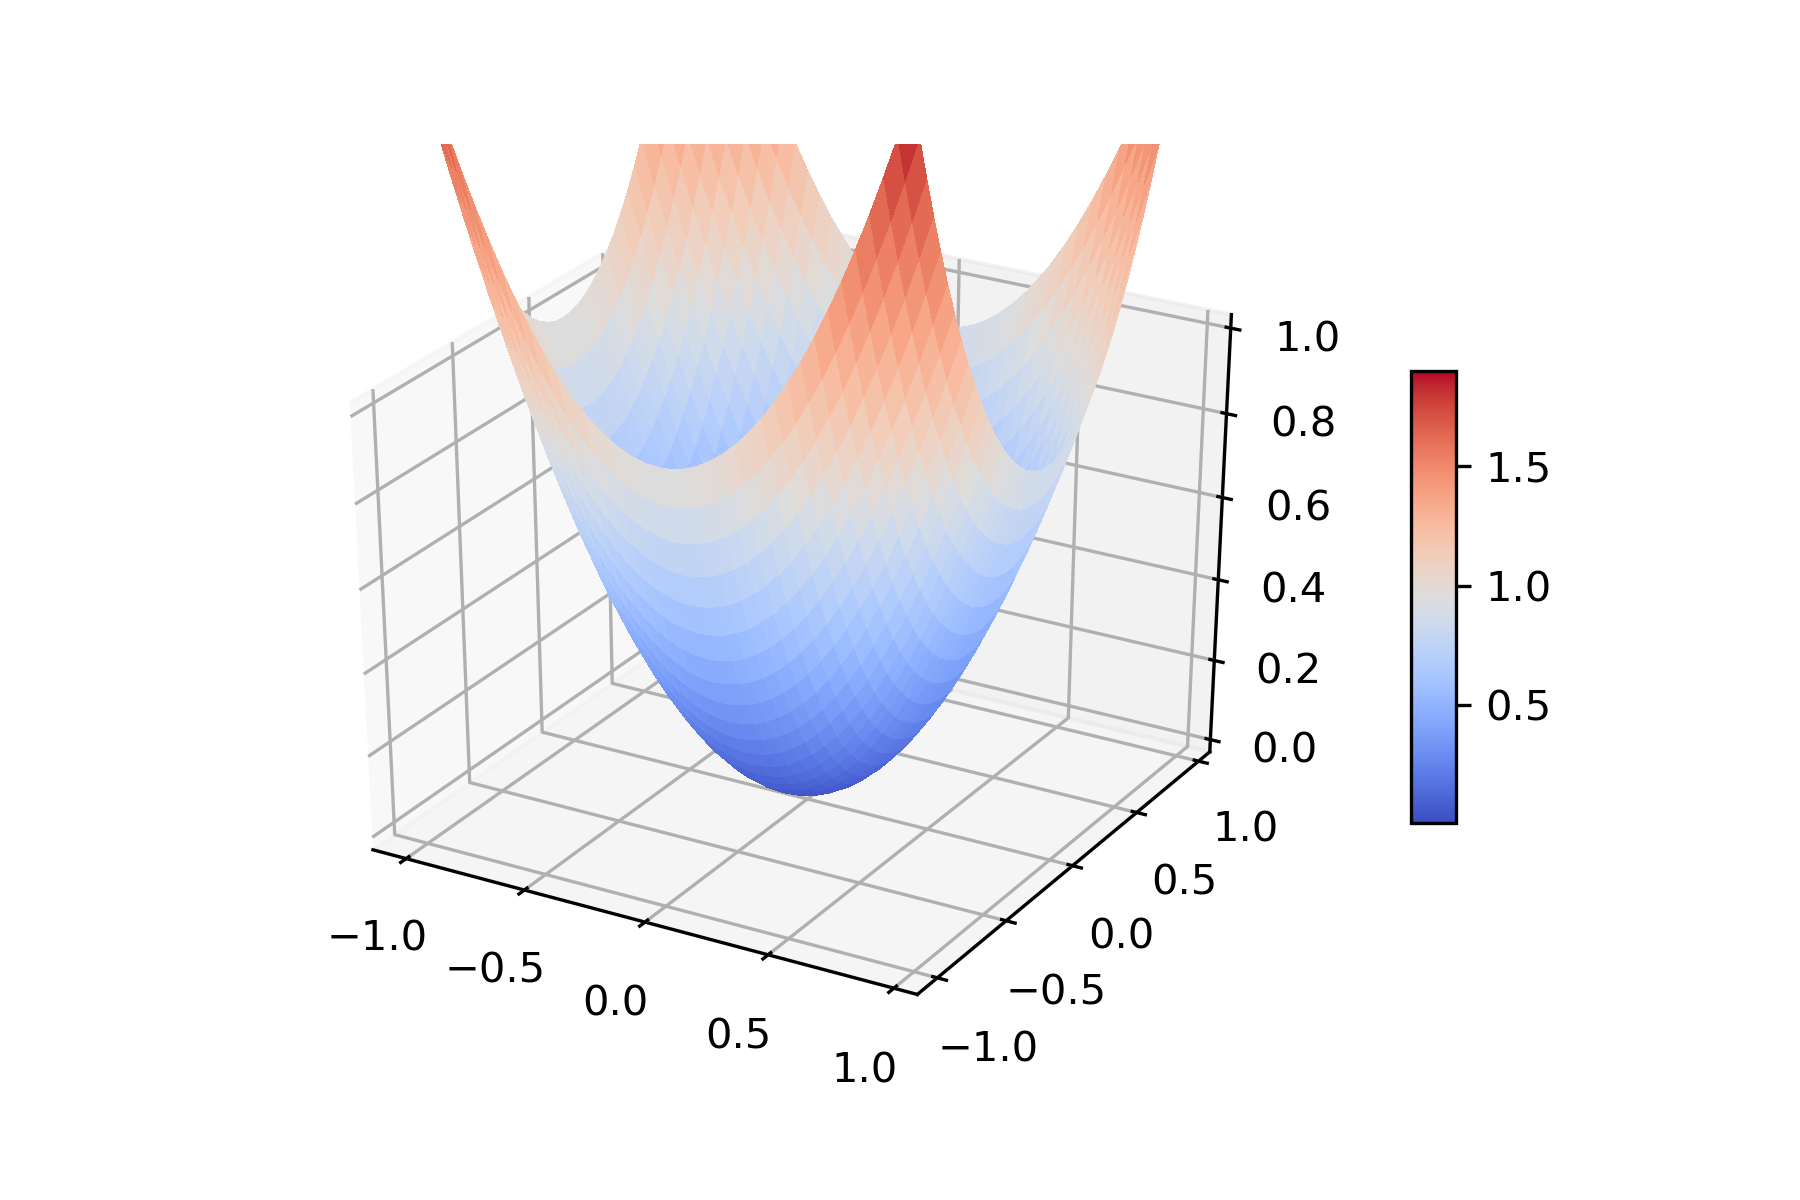
\includegraphics[scale = 0.5]{Figures/graph_positive.png}

\item Отрицательно определенная форма $z = - x^2 - y^2$.
Начало координат -- точка максимума.

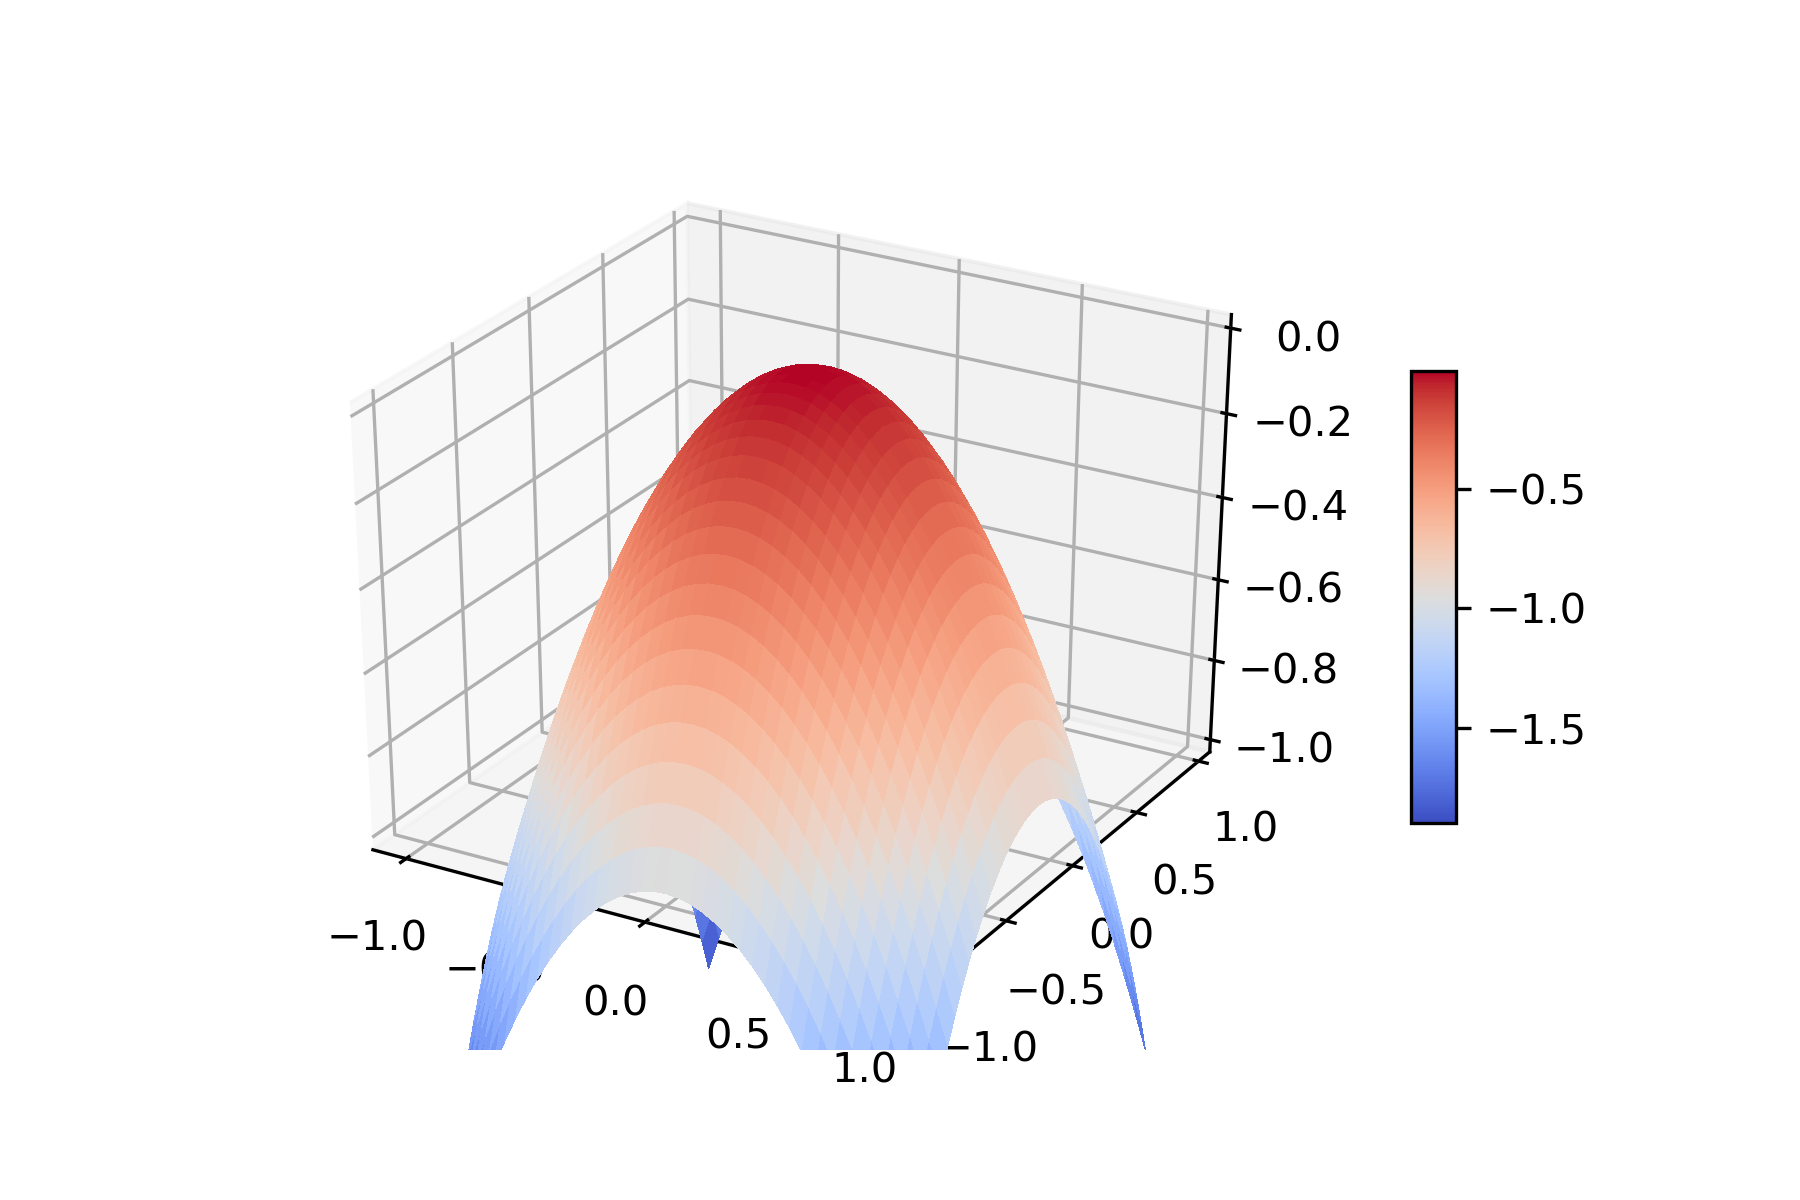
\includegraphics[scale = 0.5]{Figures/graph_negative.png}

\item Неотрицательно определенная форма $z = x^2$.
Минимум достигается на прямой $ x = 0$.

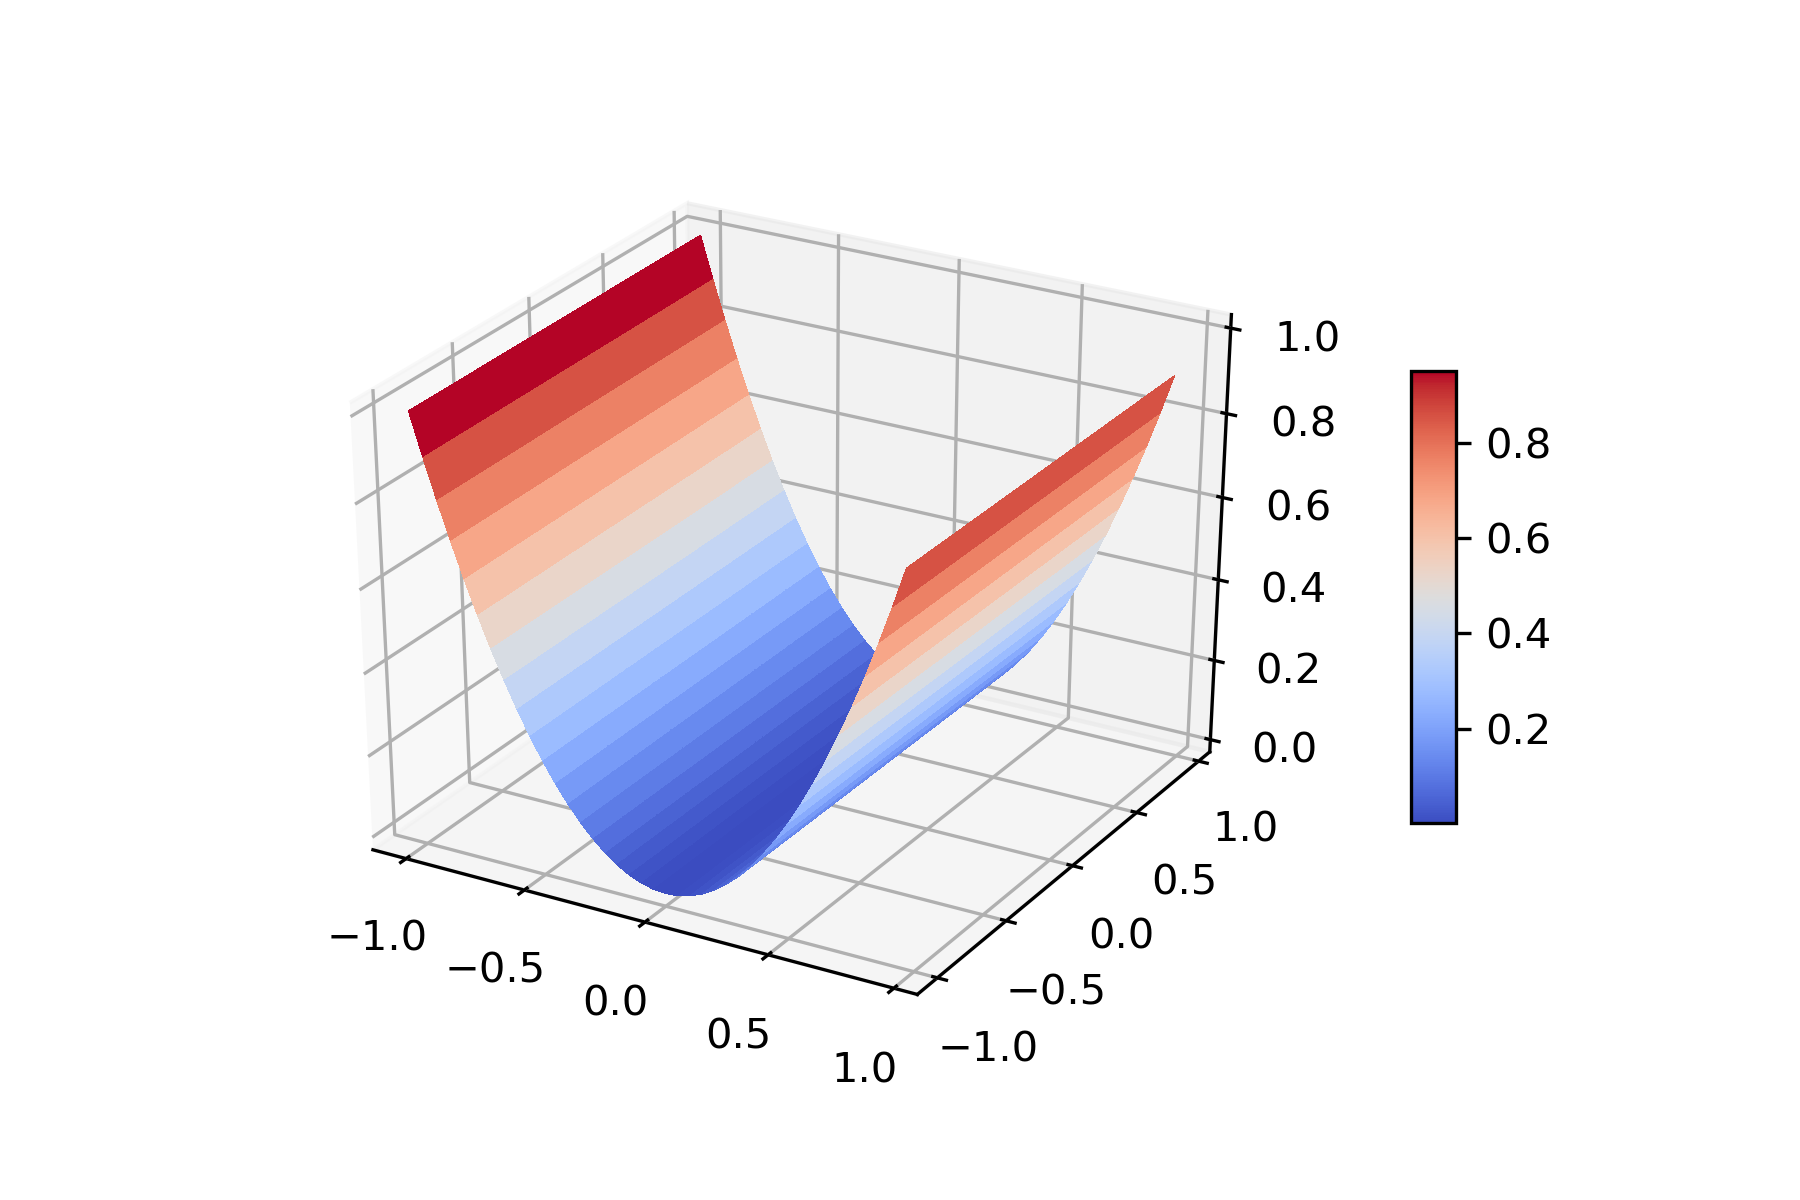
\includegraphics[scale = 0.5]{Figures/graph_non_negative.png}

\item Неположительно определенная форма $z = - x^2$.
Максимум достигается на прямой $x = 0$.

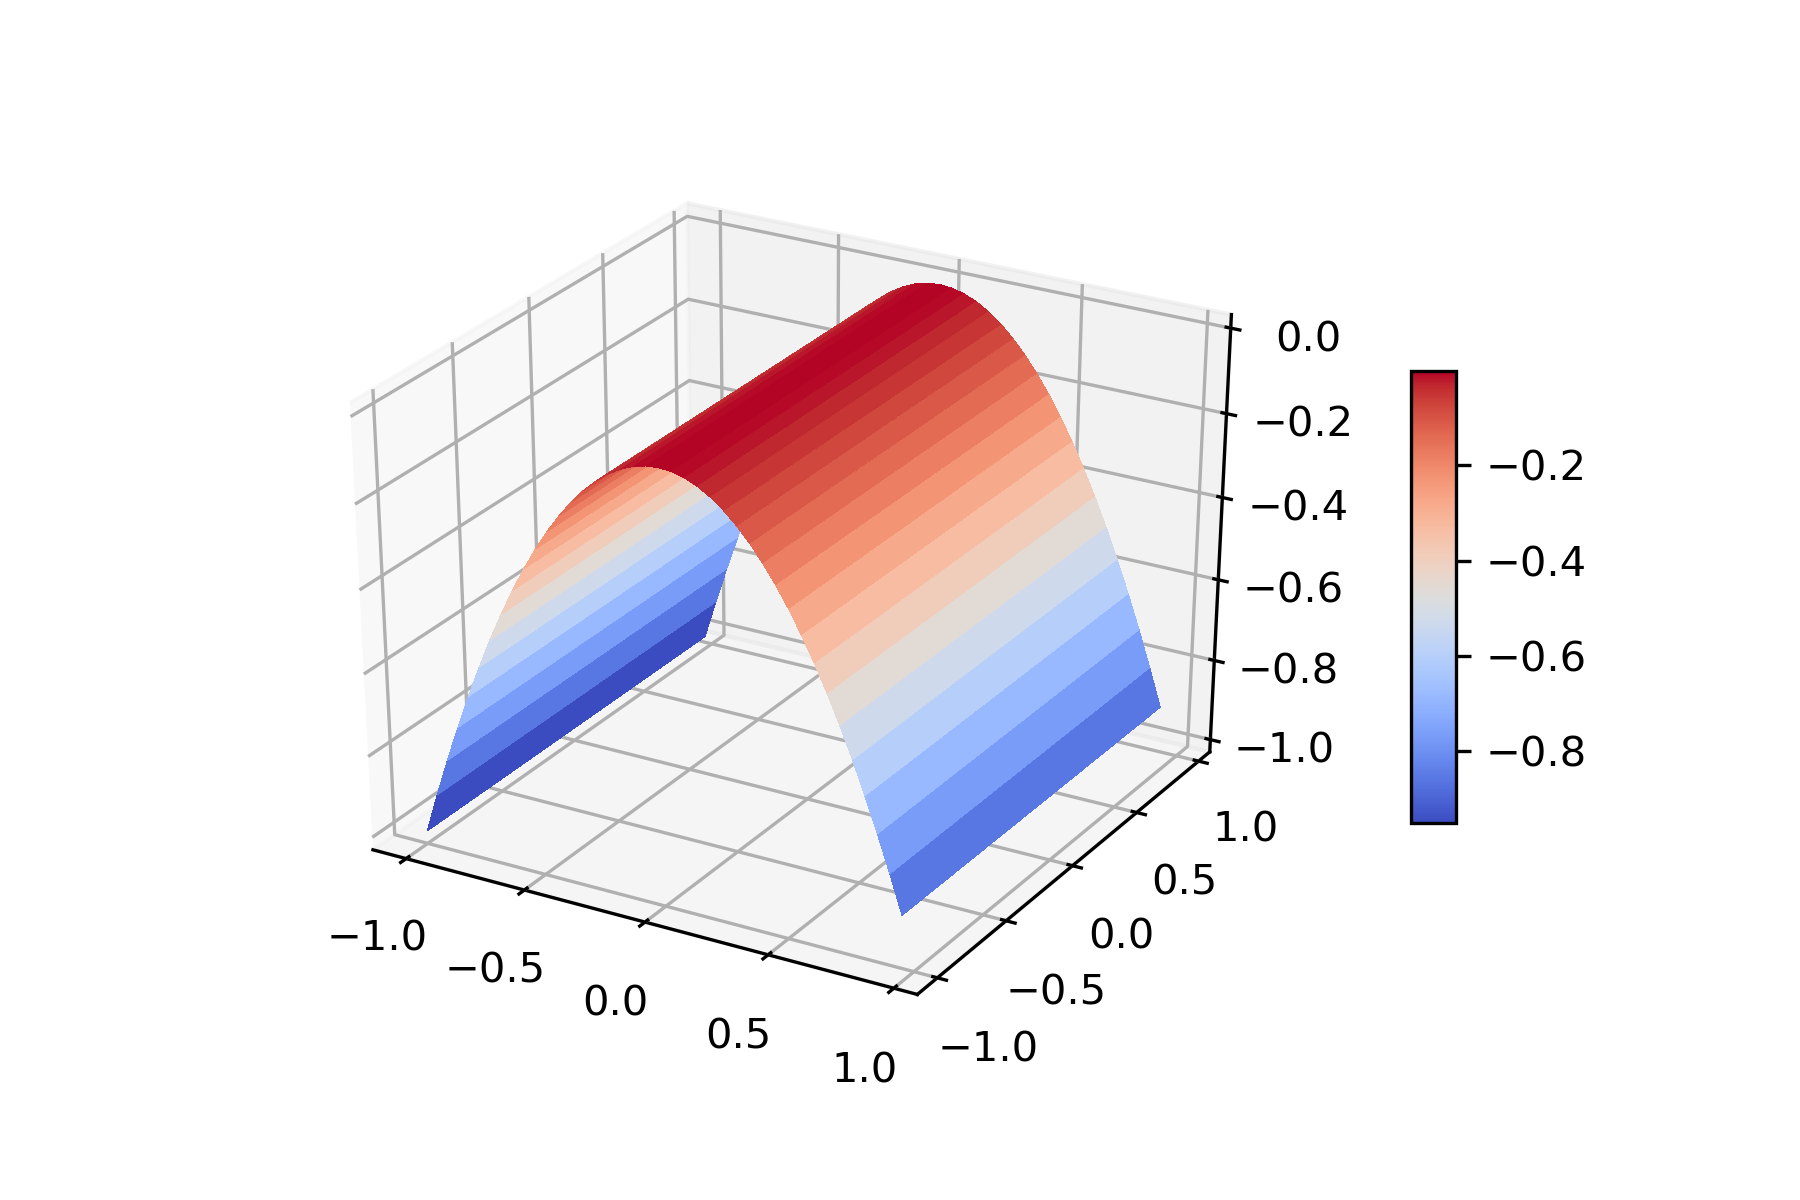
\includegraphics[scale = 0.5]{Figures/graph_non_positive.png}

\item Неопределенная форма $z = x^2 - y^2$.
Начало координат -- седловая точка.

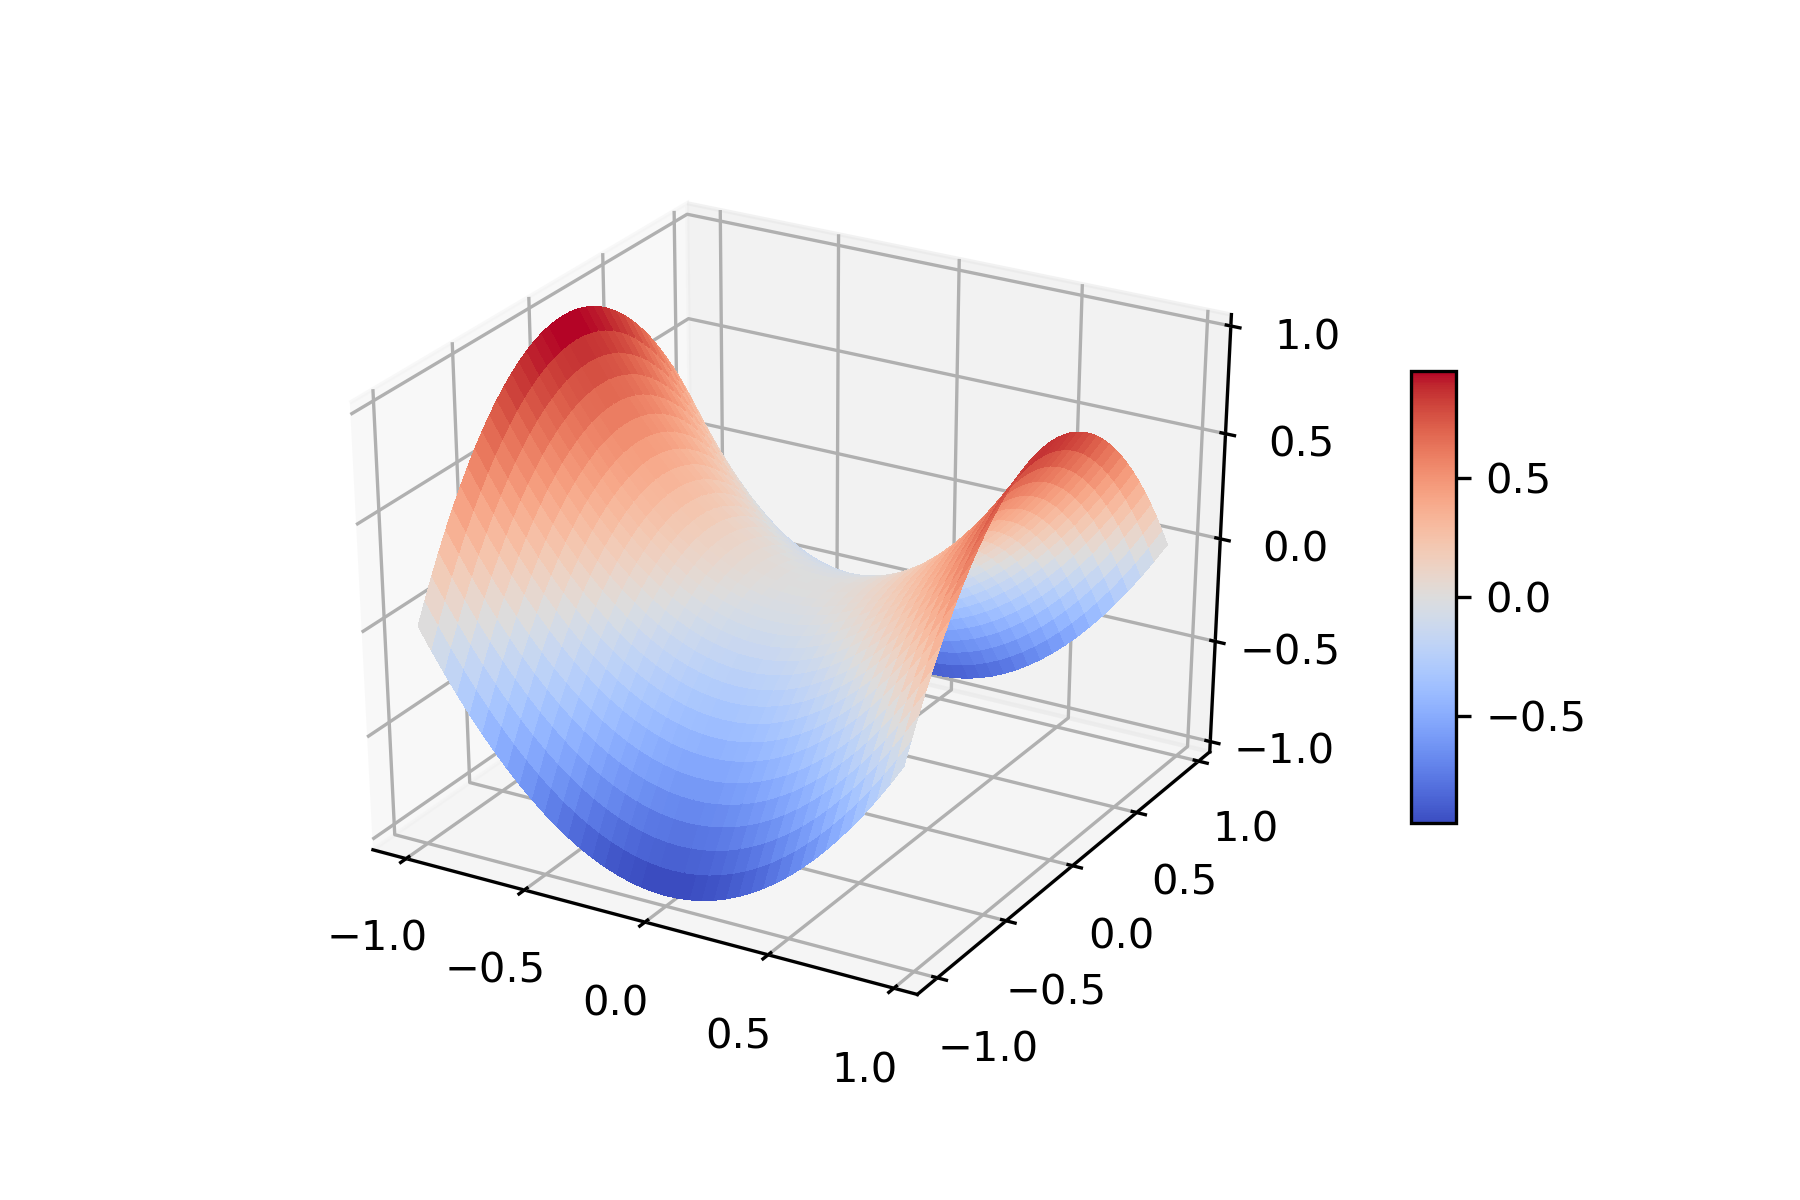
\includegraphics[scale = 0.5]{Figures/graph_saddle.png}
\end{enumerate}


\subsection{Анализ поверхности}

Квадратичные формы применяются для анализа поверхности графика функции от многих переменных.
Давайте я вкратце обрисую как.
Пусть $f\in C^2(\mathbb R^n)$ -- функция $n$ переменных, дифференцируемая дважды и вторые производные все непрерывны.
Тогда для любой точки $a\in \mathbb R^n$ выполнено разложение Тейлора
\[
f(z) = f(a) + \sum_{i=1}^n \frac{\partial f}{\partial x_i}(a)(z_i-a_i) + \sum_{ij=1}^n\frac{\partial^2 f}{\partial x_i\partial x_j}(a)(z_i-a_i)(z_j-a_j) + o(|z - a|^2)
\]
Здесь $o(|z-a|^2) = |z-a|^2 o(1)$, где $o(1)\to 0$ когда $z \to a$.
Геометрический смысл слагаемых следующий
\begin{enumerate}
\item Первое слагаемое $f(a)$ -- значение функции в точке.
Тут я никого этим не удивил.
Это лучшее приближение константой для нашей функции в точке $a$.

\item Второе слагаемое
\[
\sum_{i=1}^n \frac{\partial f}{\partial x_i}(a)(z_i-a_i)
\]
задает касательную плоскость в точке $a$ к графику функции $y = f(z)$.
То есть это линейное приближение для графика функции.
Эта плоскость горизонтальна тогда и только тогда, когда $ \frac{\partial f}{\partial x_i}(a) = 0$ для всех $1\leqslant i\leqslant n$.

\item Третье слагаемое 
\[
\sum_{ij=1}^n\frac{\partial^2 f}{\partial x_i\partial x_j}(a)(z_i-a_i)(z_j-a_j)
\]
является квадратичным приближением для графика функции.
Матрица с коэффициентами $\frac{\partial^2 f}{\partial x_i\partial x_j}(a)$ задает квадратичную форму называемую гессианом.
Если касательная плоскость горизонтальна, то сигнатура этой квадратичной формы определяет поведение графика в окрестности точки.
\begin{itemize}
\item Если форма положительно определена, то это точка локального минимума.

\item Если форма отрицательно определена, то это точка локального максимума.

\item Если форма не вырождена и неопределена, то это седловая точка
\end{itemize}
\end{enumerate}


\newpage
\section{Евклидовы пространства}

\subsection{Определение и примеры}

\begin{definition}
Евклидово пространство -- это пара $V$ и $({-},{-})$, где 
\begin{itemize}
\item $V$ -- векторное пространство над полем $\mathbb R$.

\item $({-},{-})\colon V\times V\to \mathbb R$ -- билинейная форма
\end{itemize}
При этом выполнены следующие аксиомы:
\begin{enumerate}
\item Форма $({-},{-})$ симметрическая.

\item Форма $({-},{-})$ положительно определена.
\end{enumerate}
Такая билинейная форма называется скалярным произведением.
\end{definition}

Очень часто, для краткости, когда задано евклидово пространство $V, ({-},{-})$, говорят, что $V$ является евклидовым пространством, подразумевая, что на нем есть скалярное произведение.

\paragraph{Примеры}

\begin{enumerate}
\item Пространство $\mathbb R^n$ со стандартным скалярным произведением $(x,y) = x^t y$.
Тогда $Q(x) = x^t x = \sum_{i=1}^n x_i^2 > 0$ при $x\neq 0$.

\item Пространство $\Matrix{n}$ со скалярным произведением $(A, B) = \tr(A^t B)$.
Тогда $Q(A) = \tr(A^t A) = \sum_{i,j=1}^n a_{ij}^2 > 0$ при $A\neq 0$.

\item Пусть $C[0,1]$ -- пространство непрерывных функций на отрезке $[0,1]$ сл скалярным произведением $(f,g) = \int_0^1 f(x) g(x)\,dx$.
Тогда $Q(f) = \int_0^1 f^2(x)\,dx > 0$ при $f \neq 0$.%
\footnote{В силу непрерывности, если $f(x)\neq 0$, то в какой-то окрестности $(x-\delta, x+\delta)$ точки $x$ имеем $|f(y)| > |f(x)| - \varepsilon$.}
\end{enumerate}

Важный вопрос: а как задавать скалярные произведения на некотором пространстве $V$?
Если в $V$ выбрать базис, то оно превратится в $\mathbb R^n$.
Тогда скалярное произведение задается симметричной матрицей $B$ с положительной сигнатурой.
Самый неудобный момент здесь заключается в том, что вообще говоря, глядя на матрицу $B$ не очевидно является ли она положительно определенной или нет.
Для этого надо пользоваться критерием Сильвестра (утверждение~\ref{claim::SilvCrit}).
Оказывается есть способ лучше, его мы обсудим далее.


\subsection{Ортогональные и ортонормированные базисы}

\begin{definition}
Пусть $V$ -- евклидово пространство.
Тогда
\begin{itemize}
\item Набор $v_1,\ldots,v_k\in V$ называется ортогональным, если $(v_i,v_j) = 0$ для всех $i\neq j$.

\item Набор $v_1,\ldots,v_k\in V$ называется ортонормированным, если он ортогонален и $(v_i,v_i) = 1$ для любого $i$.
\end{itemize}
Если $e_1,\ldots,e_n$ -- базис $V$, то он называется ортогональным или ортонормированным базисом, если набор $e_1,\ldots,e_n$ ортогонален или ортонормирован.
\end{definition}

\paragraph{Замечания}

\begin{itemize}
\item Базис является ортогональным тогда и только тогда, когда матрица скалярного произведения в нем диагональная.

\item Базис является ортонормированным тогда и только тогда, когда матрица скалярного произведения в нем единичная.

\item Утверждение~\ref{claim::SBilReal} говорит, что матрицу скалярного произведения всегда можно привести к единичной в некотором базисе.
То есть ортонормированные базисы существуют.

\item Процесс применяемый в методе Якоби (раздел~\ref{subsection::JacobyAlg}) превращает любой базис в ортогональный.%
\footnote{В евклидовых пространствах этот процесс называется процессом ортогонализации Грама-Шмидта.
Определение будет дальше.}
\end{itemize}


\begin{claim}
\label{claim::ScalarDef}
Пусть $V$ -- векторное пространство над $\mathbb R$.
Тогда для любого базиса $e_1,\ldots,e_n$ существует единственное скалярное произведение $({-},{-})$ на $V$ такое, что $e_1,\ldots,e_n$ является ортонормированным базисом.
\end{claim}
\begin{proof}
Зафиксируем базис $e_1,\ldots,e_n$.
Тогда задать билинейную форму -- это все равно, что задать матрицу $B\in \Matrix{n}$ (утверждение~\ref{claim::BilinearMatrices}).
Когда такая матрица $B$ задает скалярное произведение, в котором $e_1,\ldots,e_n$ -- ортонормированный базис?
Тогда и только тогда, когда $B = E$.
\end{proof}

По ортогональным и ортонормированным базисам удобно раскладывать произвольные векторы.

\begin{claim}
Пусть $V$ -- евклидово пространство, $e_1,\ldots,e_n$ -- базис и $v\in V$ -- произвольный вектор.
Тогда
\begin{enumerate}
\item Если $e_1,\ldots,e_n$ ортогональный, то 
\[
v = \frac{(v,e_1)}{(e_1,e_1)}e_1 + \ldots + \frac{(v,e_n)}{(e_n,e_n)} e_n
\]

\item Если $e_1,\ldots,e_n$ ортонормированный, то
\[
v = (v,e_1)e_1+\ldots+(v,e_n)e_n
\]
\end{enumerate}
\end{claim}
\begin{proof}
Вторая формула есть элементарное следствие первой, так как $(e_i,e_i) = 1$ для ортонормированного базиса.
Потому достаточно доказать первую формулу.
Пусть $v = \alpha_1e_1+\ldots+\alpha_n e_n$.
Умножим скалярно левую и правую часть на вектор $e_k$, тогда получим $(v, e_k) = \sum_{i=1}^n \alpha_i(e_i, e_k) = \alpha_k (e_k,e_k)$.
Значит, $\alpha_k = \frac{(v,e_k)}{(e_k,e_k)}$, что и требовалось.
\end{proof}


\begin{claim}
Пусть $A\in \Matrix{n}$.
Тогда следующие условия равносильны
\begin{enumerate}
\item $A^t A = E$.

\item $AA^t = E$.

\item $A^t = A^{-1}$.
\end{enumerate}
\end{claim}
\begin{proof}
Это следует из существования и единственности обратного при наличии левого или правого обратного (утверждение~\ref{claim::InvertibleDiscription}).
\end{proof}

\begin{definition}
Матрица $A\in \Matrix{n}$ называется ортогональной, если выполнено одно из эквивалентных свойств из предыдущего утверждения, например, $A^t A = E$.
\end{definition}

\paragraph{Замечание}

Рассмотрим в $\mathbb R^n$ стандартное скалярное произведение.
Если $A\in\Matrix{n}$, то условие $A^t A = E$ означает, что столбцы матрицы $A$ образуют ортонормированный базис.
Условие $A A^t = E$ означает, что строки матрицы $A$ образуют ортонормированный базис.
Важно понимать, что эти условия эквивалентны.
А именно, если вы возьмете ортонормированный базис в $\mathbb R^n$ и поставите эти векторы в столбцы матрицы $A$, то строки этой матрицы автоматически образуют некий другой ортонормированный базис в $\mathbb R^n$.

\begin{claim}
\label{claim::OrthoBasisDiscrEucl}
Пусть $V$ -- евклидово пространство.
Тогда
\begin{enumerate}
\item Если $e_1,\ldots,e_n$ и $f_1,\ldots,f_n$ -- два ортонормированных базиса, то матрица перехода между ними будет ортогональна.

\item Если $e_1,\ldots,e_n$ -- ортонормированный базис и $C\in \Matrix{n}$ -- ортогональная матрица, то базис $(e_1,\ldots,e_n)C$ будет ортонормированным.
\end{enumerate}
\end{claim}
\begin{proof}
(1) Пусть $(f_1,\ldots,f_n) = (e_1,\ldots,e_n)C$, где $C\in \Matrix{n}$.
Так оба базиса ортонормированные, то матрица скалярного произведения в каждом из этих базисов единичная.
По правилу изменения матрицы билинейной формы при смене базиса получаем $E = C^t E C$.
Значит $C$ ортогональная.

(2) Пусть $(f_1,\ldots,f_n) = (e_1,\ldots,e_n)C$.
В базисе $e_1,\ldots,e_n$ матрица билинейной формы $E$, так как он ортонормированный.
Матрица в базисе $f_1,\ldots,f_n$ будет $C^t E C$.
Так как $C$ ортогональная, то это будет $E$, то есть $f_1,\ldots,f_n$ -- ортонормированный базис.
\end{proof}

Таким образом за переход между ортонормированными базисами отвечают только ортогональные матрицы.

\subsection{Классификация Евклидовых пространств}

Если у нас есть два векторных пространства $V$ и $U$, то они изоморфны (то есть по сути одно и то же векторное пространство, но заданное по-разному) тогда и только тогда, когда у них одинаковые размерности (утверждение~\ref{claim::VectorClassific}).
Теперь мы хотим решить ту же самую задачу для евклидовых пространств -- понять, когда они будут одинаковыми.
Для начала надо объяснить, что значит изоморфизм евклидовых пространств.

\begin{definition}
Пусть $V$ и $U$ -- два евклидовых пространства.
Линейное отображение $\phi\colon V\to U$ называется изоморфизмом евклидовых пространств, если
\begin{enumerate}
\item $\phi$ -- изоморфизм векторных пространств.

\item Для любых $v,u\in V$ выполнено $(v, u) = (\phi(v), \phi(u))$.%
\footnote{Здесь слева скалярное произведение в пространстве $V$, а с права в пространстве $U$.}
\end{enumerate}
При наличии изоморфизма между евклидовыми пространствами $V$ и $U$ они называются изоморфными.
\end{definition}

Второе условие в определении можно выразить коммутативностью следующей диаграммы
\[
\xymatrix@R=6pt@C=40pt{
	{V\times V}\ar[dd]^{\phi\times \phi}\ar[rd]&{}&{(v,u)}\ar@{|->}[dd]\ar@{|->}[rd]&{}\\
	{}&{\mathbb R}&{}&{(v,u) = (\phi(v),\phi(u))}\\
	{U\times U}\ar[ru]&{}&{(\phi(v),\phi(u))}\ar@{|->}[ru]&{}
}
\]
Смысл определения в том, что при изоморфизме не только вектора и операции над ними переходят в соответствующие вектора и операции, но и скалярное произведение на первом пространстве превращается в скалярное произведение на втором после применения измоморфизма.
Значит при таком изоморфизме вся структура евклидова пространства сохраняется, а значит мы считаем, что такие пространства одинаковые, как евклидовы пространства.
Более того, все свойства таких пространств (если они выражены в терминах евклидова пространства) одинаковые и одно можно безболезненно менять на другое, если это удобно.


\begin{claim}
\label{claim::EuclideanIsom}
Два евклидовых пространства $V$ и $U$ изоморфны тогда и только тогда, когда $\dim V = \dim U$.
\end{claim}
\begin{proof}
Ясно, что у изоморфных пространств одинаковая размерность.
Потому надо показать, что из условия $\dim V = \dim U$ найдется изоморфизм, согласованный со скалярным произведением.
Давайте выберем ортонормированный базис $e_1,\ldots,e_n$ в $V$ и ортонормированный базис $f_1,\ldots,f_n$ в $U$.
Тогда построим линейное отображение $\phi\colon V\to U$ отправляющее $e_i\mapsto f_i$ (такое найдется единственное по утверждению~\ref{claim::LinMapExist}).
Если векторы $v,u\in V$ имеют координаты $x,y\in \mathbb R^n$ в базисе $e_1,\ldots,e_n$, то векторы $\phi(v),\phi(u)\in U$ имеют те же самые координаты $x,y$ в базисе $f_1,\ldots,f_n$.
Тогда $(v,u) = x^ty$ и $(\phi(v),\phi(u)) = x^ty$.
\end{proof}

\paragraph{Замечания}

\begin{itemize}
\item Таким образом добавление скалярного произведения к пространству не увеличивает количество не изоморфных векторных пространств.

\item Пространство $\mathbb R^2$ со стандартным скалярным произведением является <<школьной плоскостью>>, которую мы все долго и упорно изучали в курсе геометрии школьной программы.
А пространство $\mathbb R^3$ со стандартным произведением является <<школьным пространством>>.

\item Самым важным с идейной точки зрения является следующее наблюдение, которое вытекает из предыдущего утверждения.
Пусть мы хотим доказать что-то про два вектора $v,u\in V$ в каком-то евклидовом пространстве.
Тогда они обязательно содержатся в каком-то двумерном подпространстве $U\subseteq V$.
Само $U$ тоже является евклидовым вместе с ограничением скалярного произведения с $V$.
Но у нас есть школьная плоскость, которая тоже является двумерным евклидовым пространством.
А значит, это то же самое пространство, что и $U$.
То есть нам достаточно доказать факт для произвольных двух векторов на школьной плоскости.
Получается, что автоматически можно пользоваться результатами школьной геометрии.
Аналогичная идея работает с тремя векторами и сведением задачи к школьной стереометрии.

\item Несмотря на то, что можно пользоваться школьной геометрией, бывает полезно понять, как именно доказывать те или иные утверждения пользуясь формализмами линейной алгебры напрямую.
Потому я буду периодически демонстрировать какие-то вещи в лоб.
\end{itemize}
